\StartOf{Lecture 12}

\Today{ (1) Probability of Error in $M$-ary PAM}

\announcements{
\begin{itemize}
  \item Today:  Rice 6.1; Wed 3/4: Rice 6.2.
  \item Office Hours for Keren Li: 4-5pm today.  Neal: Friday 9:15am-10:15am
  \item Homework 5 due today
  \item Exam 1 on Monday 3/2 in class
  \item Project 4 due Wed 3/4
\end{itemize}
}




\section{Review of $N$-D Detection Theory with Multiple Symbols}

For $M$-ary signals, we discussed how the lowest probability of error, or \emph{Bayesian optimal}, detector finds the maximum joint probability, among the $M$ possible hypotheses $H_m$, for $m=1, \ldots, M$:
\begin{eqnarray}
  H_0: && f_{X|H_0}(x| H_0) \PR{H_0} \nonumber \\
  H_1: && f_{X|H_1}(x| H_1) \PR{H_1} \nonumber \\
  \cdots && \cdots \nonumber \\
  H_{M-1}: && f_{X|H_{M-1}}(x| H_{M-1}) \PR{H_{M-1}} \nonumber
\end{eqnarray}
The receiver finds which of these joint probabilities is highest.  For equally probable
symbols, additive Gaussian noise with identical variance in each $H_m$,
\[
  \mbox{Symbol Decision} = \arg \max_i \| \mbx - \mba_i \|
\]


\section{$M$-ary PAM Probability of Error}

\begin{figure}[htbp]
  \centerline{ 


\tikzset{every picture/.style={line width=0.75pt}} %set default line width to 0.75pt        

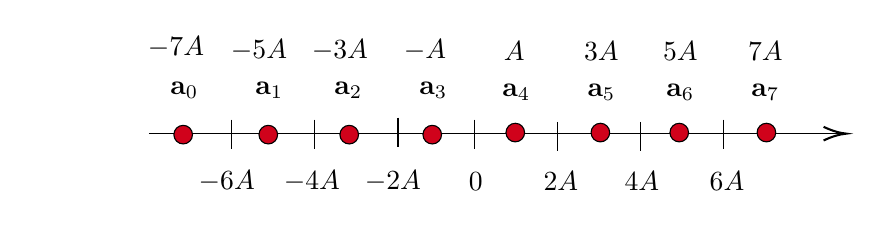
\begin{tikzpicture}[x=0.75pt,y=0.75pt,yscale=-1,xscale=1]
%uncomment if require: \path (0,300); %set diagram left start at 0, and has height of 300

%Straight Lines [id:da0785677110363594] 
\draw    (173.96,114) -- (507.96,114) ;
\draw [shift={(509.96,114)}, rotate = 180] [color={rgb, 255:red, 0; green, 0; blue, 0 }  ][line width=0.75]    (10.93,-3.29) .. controls (6.95,-1.4) and (3.31,-0.3) .. (0,0) .. controls (3.31,0.3) and (6.95,1.4) .. (10.93,3.29)   ;

%Shape: Circle [id:dp8429373004294252] 
\draw  [fill={rgb, 255:red, 208; green, 2; blue, 27 }  ,fill opacity=1 ] (306,114.48) .. controls (306,112.01) and (308.01,110) .. (310.48,110) .. controls (312.96,110) and (314.96,112.01) .. (314.96,114.48) .. controls (314.96,116.96) and (312.96,118.96) .. (310.48,118.96) .. controls (308.01,118.96) and (306,116.96) .. (306,114.48) -- cycle ;
%Straight Lines [id:da9917337286598218] 
\draw    (330.96,107.29) -- (330.96,121.29) ;


%Shape: Circle [id:dp31317929420387847] 
\draw  [fill={rgb, 255:red, 208; green, 2; blue, 27 }  ,fill opacity=1 ] (266,114.48) .. controls (266,112.01) and (268.01,110) .. (270.48,110) .. controls (272.96,110) and (274.96,112.01) .. (274.96,114.48) .. controls (274.96,116.96) and (272.96,118.96) .. (270.48,118.96) .. controls (268.01,118.96) and (266,116.96) .. (266,114.48) -- cycle ;
%Shape: Circle [id:dp8703696009425539] 
\draw  [fill={rgb, 255:red, 208; green, 2; blue, 27 }  ,fill opacity=1 ] (227,114.48) .. controls (227,112.01) and (229.01,110) .. (231.48,110) .. controls (233.96,110) and (235.96,112.01) .. (235.96,114.48) .. controls (235.96,116.96) and (233.96,118.96) .. (231.48,118.96) .. controls (229.01,118.96) and (227,116.96) .. (227,114.48) -- cycle ;
%Shape: Circle [id:dp48312291319442124] 
\draw  [fill={rgb, 255:red, 208; green, 2; blue, 27 }  ,fill opacity=1 ] (186,114.48) .. controls (186,112.01) and (188.01,110) .. (190.48,110) .. controls (192.96,110) and (194.96,112.01) .. (194.96,114.48) .. controls (194.96,116.96) and (192.96,118.96) .. (190.48,118.96) .. controls (188.01,118.96) and (186,116.96) .. (186,114.48) -- cycle ;
%Shape: Circle [id:dp32010417887626774] 
\draw  [fill={rgb, 255:red, 208; green, 2; blue, 27 }  ,fill opacity=1 ] (467,113.48) .. controls (467,111.01) and (469.01,109) .. (471.48,109) .. controls (473.96,109) and (475.96,111.01) .. (475.96,113.48) .. controls (475.96,115.96) and (473.96,117.96) .. (471.48,117.96) .. controls (469.01,117.96) and (467,115.96) .. (467,113.48) -- cycle ;
%Shape: Circle [id:dp665622950437736] 
\draw  [fill={rgb, 255:red, 208; green, 2; blue, 27 }  ,fill opacity=1 ] (425,113.48) .. controls (425,111.01) and (427.01,109) .. (429.48,109) .. controls (431.96,109) and (433.96,111.01) .. (433.96,113.48) .. controls (433.96,115.96) and (431.96,117.96) .. (429.48,117.96) .. controls (427.01,117.96) and (425,115.96) .. (425,113.48) -- cycle ;
%Shape: Circle [id:dp5860873971209044] 
\draw  [fill={rgb, 255:red, 208; green, 2; blue, 27 }  ,fill opacity=1 ] (387,113.48) .. controls (387,111.01) and (389.01,109) .. (391.48,109) .. controls (393.96,109) and (395.96,111.01) .. (395.96,113.48) .. controls (395.96,115.96) and (393.96,117.96) .. (391.48,117.96) .. controls (389.01,117.96) and (387,115.96) .. (387,113.48) -- cycle ;
%Shape: Circle [id:dp20437801267978872] 
\draw  [fill={rgb, 255:red, 208; green, 2; blue, 27 }  ,fill opacity=1 ] (346,113.48) .. controls (346,111.01) and (348.01,109) .. (350.48,109) .. controls (352.96,109) and (354.96,111.01) .. (354.96,113.48) .. controls (354.96,115.96) and (352.96,117.96) .. (350.48,117.96) .. controls (348.01,117.96) and (346,115.96) .. (346,113.48) -- cycle ;
%Straight Lines [id:da51291390000777] 
\draw    (370.96,108.29) -- (370.96,122.29) ;


%Straight Lines [id:da2811648906641422] 
\draw    (410.96,108.29) -- (410.96,122.29) ;


%Straight Lines [id:da4403380546942397] 
\draw    (450.96,107.29) -- (450.96,121.29) ;


%Straight Lines [id:da9495765085027235] 
\draw    (213.96,107.29) -- (213.96,121.29) ;


%Straight Lines [id:da24674873474006298] 
\draw    (253.96,107.29) -- (253.96,121.29) ;


%Straight Lines [id:da44203695518931974] 
\draw    (293.96,106.29) -- (293.96,120.29) ;



% Text Node
\draw (331.48,136.96) node   {$0$};
% Text Node
\draw (120,142) node   {$$};
% Text Node
\draw (191,93) node   {$\mathbf{a}_{0}$};
% Text Node
\draw (232,93) node   {$\mathbf{a}_{1}$};
% Text Node
\draw (270,93) node   {$\mathbf{a}_{2}$};
% Text Node
\draw (311,93) node   {$\mathbf{a}_{3}$};
% Text Node
\draw (351,94) node   {$\mathbf{a}_{4}$};
% Text Node
\draw (392,94) node   {$\mathbf{a}_{5}$};
% Text Node
\draw (430,94) node   {$\mathbf{a}_{6}$};
% Text Node
\draw (471,94) node   {$\mathbf{a}_{7}$};
% Text Node
\draw (187,72.5) node   {$-7A$};
% Text Node
\draw (227,74) node   {$-5A$};
% Text Node
\draw (266,74) node   {$-3A$};
% Text Node
\draw (307,74) node   {$-A$};
% Text Node
\draw (350,74) node   {$A$};
% Text Node
\draw (392,74) node   {$3A$};
% Text Node
\draw (430,74) node   {$5A$};
% Text Node
\draw (471,74) node   {$7A$};
% Text Node
\draw (372.48,136.96) node   {$2A$};
% Text Node
\draw (411.48,136.96) node   {$4A$};
% Text Node
\draw (452.48,136.96) node   {$6A$};
% Text Node
\draw (211.48,136.96) node   {$-6A$};
% Text Node
\draw (252.48,136.96) node   {$-4A$};
% Text Node
\draw (291.48,136.96) node   {$-2A$};


\end{tikzpicture}

}
  \caption{Signal space diagrams for 8-PAM, with optimal detection thresholds.}
  \label{F:8PAM_detection_thresholds}
\end{figure}

Consider $M$-PAM.  Our goal in this section is to find a formula for the probability that our optimal receiver makes a symbol error when receiving.

\subsection{Symbol Error}

The probability that we don't get the symbol correct is the
probability that $x$ does not fall within the range between the
thresholds in which it belongs.  Here, each $\mba_i = -7A + i(2A)$.  Also the
noise $\sigma_W^2 = N_0/2$, as described in our lecture on thermal noise.

Let's consider symbol $i=1$.  Recall $\mba_1 = -5A$.  The probability of error is the sum of the probability of deciding $H_0$, plus the probability of deciding $H_i$ for $i=2, \ldots, 7$.  That is, that the $x$ value is below $-6A$, or above $-4A$.  Thus
\begin{eqnarray}
  P(\mbox{symbol error}| H_1) 
    &=& \Q{\frac{-5A - (-6A) }{\sqrt{N_0/2}}} + \Q{\frac{-4A - (-5A) }{\sqrt{N_0/2}}}
  \nnn 
    &=& 2 \Q{\frac{A }{\sqrt{N_0/2}}}.
\end{eqnarray}

Assuming neighboring symbols $a_i$ are spaced by $2A$, the decision
threshold is always $A$ away from the symbol values. For the symbols
$i$ in the `middle',
\[
  P(\mbox{symbol error}| H_i) = 2 \Q{\frac{A }{\sqrt{N_0/2}}}
\]
For the symbols $i$ on the `sides',
\[
  P(\mbox{symbol error}| H_i) = \Q{\frac{A }{\sqrt{N_0/2}}}
\]
Since each symbol $H_i$ is equally likely, the overall probability of symbol error is the average of the conditional probabilities of symbol error.  That is:
\[
  P(\mbox{symbol error}) = \frac{1}{M} \sum_{i=0}^{M-1} P(\mbox{symbol error}| H_i)
\]
So overall,
\[
  P(\mbox{symbol error}) = \frac{2(M-1)}{M} \Q{\frac{A }{\sqrt{N_0/2}}}
\]

\noindent {\bf Symbol Error Rate and Average Bit Energy}:

How does this relate to the average bit energy $\En_b$?  We calculated in an earlier lecture the average symbol error for $M$-PAM as
\[
\En_s = \frac{(M^2-1)}{3} A^2
\]
But there are $\log_2 M$ bits per symbol.  We're going to want to express energy per bit instead of average energy per symbol.  Thus we use $\En_b$ to denote the average energy per bit.  Thus
\begin{equation}
\En_b = \frac{1}{\log_2 M} \frac{(M^2-1)}{3} A^2,    
\end{equation}
which means that
\[
A  = \sqrt{\frac{3 \log_2 M}{M^2-1}} \En_b
\]
So
\begin{equation} \label{E:PrSymbolErrorMPAM2}
  P(\mbox{symbol error}) = \frac{2(M-1)}{M} \Q{\sqrt{\frac{6 \log_2 M}{M^2-1} \frac{\En_b}{N_0}}}
\end{equation}
Equation (\ref{E:PrSymbolErrorMPAM2}) is plotted in Figure
\ref{F:plotPerrorMaryPAM}.

  \begin{figure}[htbp]
    \centerline{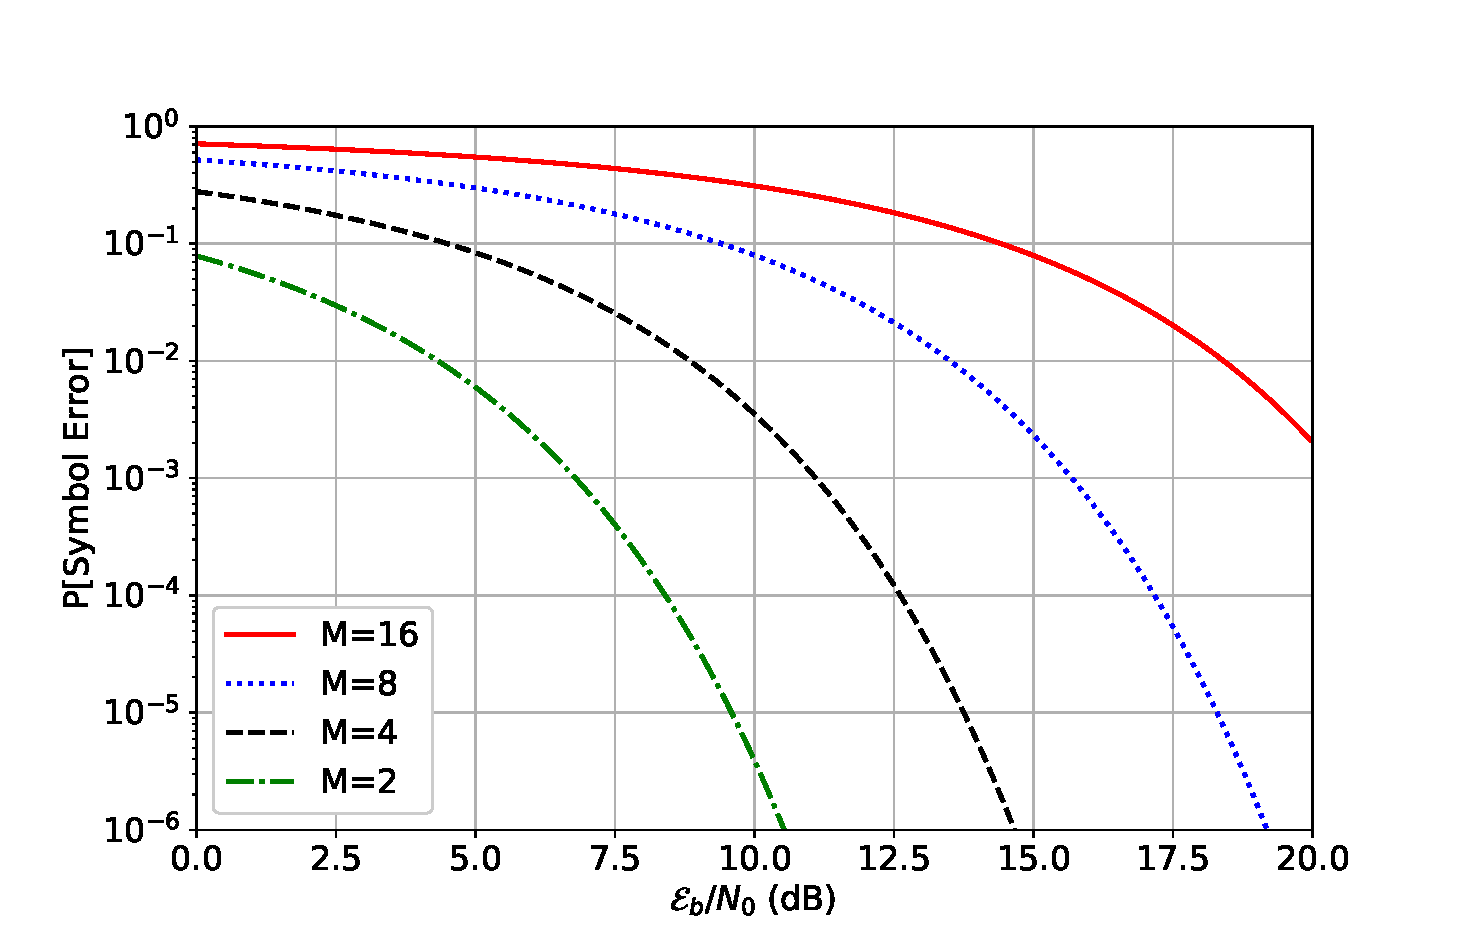
\includegraphics[width=\textwidth]{../images/plotPrSymbolErrorMPAM.eps} }
    \caption{Probability of Symbol Error in $M$-ary PAM.}
    \label{F:plotPerrorMaryPAM}
  \end{figure}


\subsection{Bit Errors and Gray Encoding}

For binary PAM, there are only two symbols, one will be assigned
binary 0 and the other binary 1.  When you make one symbol error
(decide $H_0$ or $H_1$ in error) then it will cause one bit error.

For $M$-ary PAM, bits and symbols are not synonymous.  Instead, we
carefully assign bit codes to symbols $1 \ldots M$ so that the most common receiver errors cause only one bit to be in error, and let less common receiver errors to cause more than one bit error.

\Example{Bit coding of $M=4$ symbols}  While the two options shown
in Figure \ref{F:4AryPAM-BitCodingOptions} both assign 2-bits to
each symbol in unique ways, one will lead to a higher bit error rate
than the other.  Is one is better or worse?
  \begin{figure}[htbp]
    \centerline{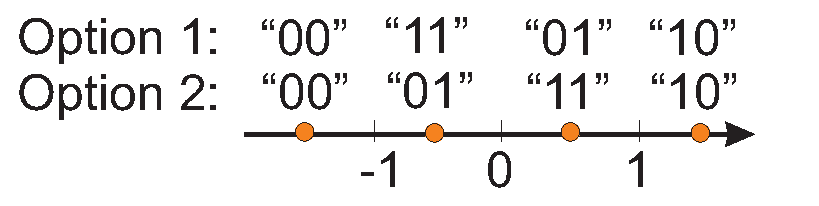
\includegraphics[width=0.5\textwidth]{../images/4AryPAM-BitCodingOptions.eps} }
    \caption{Two options for assigning bits to symbols in 4-PAM.}
    \label{F:4AryPAM-BitCodingOptions}
  \end{figure}

The key is to recall the model for noise.  It will not shift a
signal uniformly across symbols.  It will tend to leave the received
signal $x$ close to the original signal $a_i$.  The neighbors of
$a_i$ will be more likely than distant signal space vectors.

Thus Gray encoding will only change one bit across boundaries, as in
Option 2 in Figure \ref{F:4AryPAM-BitCodingOptions}.

\Example{Bit coding of $M=8$ symbols}  Assign three bits to each
symbol such that any two nearest neighbors are different in only one
bit (Gray encoding).

\Solution{Here is one solution.
  \begin{figure}[htbp]
    \centerline{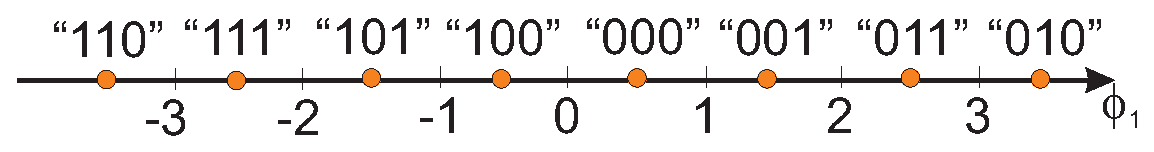
\includegraphics[width=0.6\textwidth]{../images/8AryPAM-GrayCoding.eps} }
    \caption{Gray encoding for 8-PAM.}
    \label{F:8AryPAM-GrayCoding}
  \end{figure}
}

\subsubsection{Bit Error Probabilities}

How many bit errors are caused by a symbol error in $M$-ary PAM?
\begin{itemize}
  \item One.  If Gray encoding is used, the errors will tend to be
  just one bit flipped, more than multiple bits flipped.  At least
  at high $\En_b/N_0$,
  \begin{equation} \label{E:PrBitErrorInGeneral}
    P(\mbox{error}) \approx \frac{1}{\log_2 M} P(\mbox{symbol error})
  \end{equation}
  \item Maybe more, up to $\log_2 M$ in the worst case.  Then, we
  need to study further the probability that $x$ will jump more than one decision
  region.
\end{itemize}
Generally, we study digital communications systems with high reliability, and high $\En_b/N_0$.  Thus when we calculate bit error rate for $M$-ary PAM, we
use (\ref{E:PrBitErrorInGeneral}).  We will show that this approximation is very good, in almost all cases for $M$-PAM and most common QAM/PSK modulations.  We will also discuss some particular examples in multi-dimensional signalling when this is not a great approximation.

Thus for $M$-PAM:
\begin{equation} \label{E:PrBitErrorMPAM2}
  P(\mbox{bit error}) \approx \frac{2(M-1)}{M \log_2 M} \Q{\sqrt{\frac{6 \log_2 M}{M^2-1} \frac{\En_b}{N_0}}}
\end{equation}


\section{Square QAM Probability of Error}

%This section is meant to introduce the problems we'll have as we compute the probability of symbol error in QAM and PSK, and in general, for higher dimensional symbol space diagrams.  

Consider now QAM modulation, in general, which is $N=2$.
Recall that our symbol decision is  $\arg \max_i \| \mbx - \mba_i \|$, and that this creates decision regions using a Voronoi diagram.  This can, in general, be quite complicated because we'd have a probability of error that is an integral of a 2-D Gaussian pdf in the area outside of some polygon containing $\mba_i$.  Two dimensional integrals of a Gaussian pdf aren't something for which we can find an analytical solution.  While we can solve numerically for such integrals, and people do, we tend to find easier approximations whenever possible.

Square QAM is an example where we can make the probability of symbol error formula exact, and analytical.  To do this, consider square $M$-QAM as two orthogonal $\sqrt{M}$-PAM systems.  In this case, the bits of each symbol are separated into first the bits corresponding to the in-phase component of the modulation, and next the bits corresponding to the quadrature component.  We can see that using gray coding in each component, we can arrange it so that the first bits are completely dependent on the in-phase component.  Because these $\log_2 \sqrt{M}$ bits are independent of the quadrature, the probability of bit error for these bits is the same as the the probability of bit error for $\sqrt{M}$-PAM.  Similarly, the next $\log_2 \sqrt{M}$ bits are independent of the in-phase component, and thus the probability of bit error for these bits is the same as the the probability of bit error for $\sqrt{M}$-PAM.  Overall, the probability of bit error for square $M$-QAM is equal to the probability of bit error for $\sqrt{M}$-PAM:
\begin{equation} \label{E:PrBitErrorMPAM}
  P(\mbox{bit error}) \approx \frac{4(\sqrt{M}-1)}{\sqrt{M} \log_2 M} \Q{\sqrt{\frac{3 \log_2 M}{M-1} \frac{\En_b}{N_0}}}.
\end{equation}


The probability of symbol error is the probability of a symbol error \emph{either} in the in-phase or quadrature components.  In other words, it is $1-$ the probability that we don't make an error in the in-phase, and we don't make an error in the quadrature component.  The two error events are independent so the error probabilities multiply each other.    Thus it is $1 - (1-\PR{\mbox{Symbol error in }\sqrt{M}\mbox{-PAM}})^2$, or
\[
 P(\mbox{symbol error}) = 1-\left[
   1-\frac{2(\sqrt{M}-1)}{\sqrt{M}} \Q{\sqrt{\frac{3 \log_2 M}{M-1} \frac{\En_b}{N_0}}}
 \right]^2.
\]